\documentclass[UTF8]{beamer}
\usepackage[utf8]{inputenc}
\usepackage[normalem]{ulem}
\usepackage{xeCJK}
\usepackage{
    amsmath, amssymb, listings, hyperref,
    subcaption, float, booktabs, csquotes,
    enumitem, tikz, pgf, pgfplots, cancel,
    ulem, fancyhdr, framed, amsthm, mathtools,
    ifsym
}

\setCJKmainfont[BoldFont=Songti SC Bold]{Songti SC Regular}
\setCJKsansfont{Heiti SC}
\setCJKmonofont{Courier}

\newcommand{\figc}[2]{
\begin{figure}[H]\begin{center}
    #1
    \caption{#2}
\end{center}\end{figure}
}

\usetikzlibrary{arrows, automata}
\AtBeginEnvironment{align}{\setcounter{equation}{0}}

\theoremstyle{plain}
%\newtheorem{theorem}{Theorem}
%\newtheorem*{theorem*}{Theorem}
%\newtheorem{lemma}{Lemma}


\theoremstyle{definition}
\newtheorem*{claim}{Claim}
\newtheorem{defn}{Definition}

\theoremstyle{remark}
\newtheorem{remark}{Remark}


\newcommand{\ffig}[2]{
\begin{figure}[H]\begin{center}
    #1
    \caption{#2}
\end{center}\end{figure}
}
\newcommand\m[1]{\begin{bmatrix}#1\end{bmatrix}}
\newcommand\mc[1]{\mathcal{#1}}
\newcommand\mb[1]{\mathbf{#1}}

\definecolor{dkgreen}{rgb}{0,0.6,0}
\definecolor{gray}{rgb}{0.5,0.5,0.5}
\definecolor{mauve}{rgb}{0.58,0,0.82}

\lstset{
  language=matlab,
  aboveskip=3mm,
  belowskip=3mm,
  showstringspaces=false,
  columns=flexible,
  basicstyle={\small\ttfamily},
  numbers=left,
  numberstyle=\tiny\color{gray},
  keywordstyle=\color{blue},
  commentstyle=\color{dkgreen},
  stringstyle=\color{mauve},
  breaklines=true,
  breakatwhitespace=true
  tabsize=2
}

\makeatletter
\renewcommand*\env@matrix[1][*\c@MaxMatrixCols c]{%
   \hskip -\arraycolsep
   \let\@ifnextchar\new@ifnextchar
   \array{#1}}
\makeatother

\newcommand*{\bc}{\Leftrightarrow}
\newcommand*{\then}{\Rightarrow}
\newcommand*{\st}{~\middle|~}

\newcommand*{\vrbar}{\rule[-1ex]{0.5pt}{2.5ex}}
\newcommand*{\hrbar}{\rule[.5ex]{2.5ex}{0.5pt}}

\newcommand{\zerodel}{.\kern-\nulldelimiterspace}

\newcommand{\R}{\mathbb{R}}
\renewcommand{\H}{\mathbb{H}}
\newcommand{\C}{\mathbb{C}}
\newcommand{\Z}{\mathbb{Z}}
\newcommand{\Q}{\mathbb{Q}}
\newcommand{\N}{\mathbb{N}}
\newcommand{\qedb}{$\blacksquare$}
\newcommand{\blank}{\textvisiblespace}
\newcommand{\Mod}{~\mathrm{mod}~}

\DeclareMathOperator{\Cl}{Cl}
\DeclareMathOperator{\POLY}{P}
\DeclareMathOperator{\NPOLY}{NP}
\DeclareMathOperator{\NPOLYC}{NP--Complete}
\DeclareMathOperator{\CONPOLY}{co--NP}
\DeclareMathOperator*{\argmax}{arg\,max}
\DeclareMathOperator*{\argmin}{arg\,min}
\DeclareMathOperator*{\rank}{rank}
\DeclareMathOperator*{\spn}{span}
\DeclareMathOperator*{\Arg}{Arg}
\DeclareMathOperator*{\im}{Im}
\DeclareMathOperator*{\lcm}{lcm}
\DeclareMathOperator*{\sgn}{sgn}

\DeclarePairedDelimiterX{\inp}[2]{\langle}{\rangle}{#1, #2}


\pgfplotsset{every axis/.append style={
                    axis x line=middle,    % put the x axis in the middle
                    axis y line=middle,    % put the y axis in the middle
                    axis line style={->}, % arrows on the axis
                    xlabel={$x$},          % default put x on x-axis
                    ylabel={$y$},          % default put y on y-axis
                    }}

\usefonttheme{serif}
\title{\bf Kolmogorov-Arnold Networks}
\author{jiahong.long@}
\institute{Cruise $\cdot$ UC San Diego}
\date{10 June 2024}

\begin{document}

\frame{\titlepage}

\begin{frame}
    \center{\textbf{
        Welcome to the inaugural Sim-Eval literature review!
    }}
    \center{
        I'm trying to keep this informal -- teaching is the best way of learning,
        and we all benefit from sharing knowledge. 
    }
    \center{
        My background is in math, so expect a bit more of the underlying theory here!
    }
\end{frame}

\begin{frame}
    \textbf{On the agenda:}
    \begin{itemize}
        \item MLPs and their limitations
        \item What KANs do better
        \item What KANs do worse
    \end{itemize}
\end{frame}

\begin{frame}
    Some bookkeeping notes:
    \begin{itemize}
        \item For simplicity, assume that the functions we care about are
            \textit{scalar-valued} and \textit{of multiple variables}, i.e. 
            \[
                f: \R^n \longrightarrow \R
            \]
        \item Parts of this are intentionally abstract, so as to not get
            into the weeds of technical examples. Expect a fair bit of hand-waving.
        \item The original paper is on \texttt{ArXiv:2404.19756v1}
         at \url{https://arxiv.org/pdf/2404.19756v1}.
    \end{itemize}
\end{frame}

\begin{frame}
    \center{
        \textbf{Primer:} a gentle (re)introduction to the multi-layer perceptron
    }
\end{frame}

\begin{frame}
    Canonically, a ``shallow'' multi-layer perceptron is \textit{two layers}. (This will be important
    for the literature!)
    A multi-layer perceptron in the shallow case is represented as
    \begin{align*}
        \hat{f} &: ~ \R^n \longrightarrow \R \\
        \hat{f}(x) &=  \sum_i^{N(\varepsilon)} a_i \sigma \left[\mathbf{W}_i \mathbf{x} + b_i \right]
    \end{align*}
    Note the width $N(\varepsilon)$ is a function of the precision $\varepsilon$.
\end{frame}

\begin{frame}
    \begin{align*}
        \hat{f}(x) &=  \sum_i^{N(\varepsilon)} a_i \sigma \left[\mathbf{W}_i \mathbf{x} + b_i \right]
    \end{align*}
    where:
    \[
        \begin{array}{c|l}
            b_i & \text{is the bias \textit{(affine!)}} \\
            \mathbf{x} & \text{is the $i$ th input vector} \\
            \mathbf{W}_i & \text{is the $i$ th weight matrix \textit{(learned!)}} \\
            \sigma & \text{is the activation function \textit{(e.g. ReLU, sigmoid, $\tanh$...)}} \\
            a_i & \text{are elements of the outermost weight matrix} \\
            N(\varepsilon) & \text{is the number of neurons}
        \end{array}
    \]
    In the shallow case, $a_i$ can be denoted by a row vector.
\end{frame}
\begin{frame}
    \begin{align*}
        \hat{f}(x) &=  \sum_i^{N(\varepsilon)} a_i \sigma \left[\mathbf{W}_i \mathbf{x} + b_i \right]
    \end{align*}
    \ffig{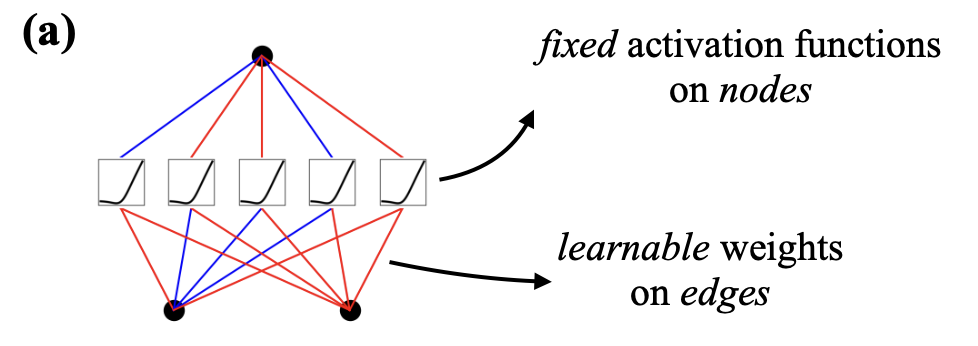
\includegraphics[width=6cm]{shallowmlp}}{\textit{A shallow 2-layer multi-layer perceptron.} $d=2$, $n=5$.}
\end{frame}
\begin{frame}
    \textit{Interesting side note:}
    more generally, for deep ($d > 2$) networks, a multi-layer perceptron is
    really just a composition of (affine!) linear transformations separated by non-linear
    activations.
    \[
        MLP(\mathbf{x}) = \left[
            \mathbf{W}_d \circ \sigma_d \circ
            \mathbf{W}_{d-1} \circ \sigma_{d-1} \circ
                \ldots
            \mathbf{W}_{1} \circ \sigma_{1} 
        \right] (\mathbf{x} )
    \]
    \ffig{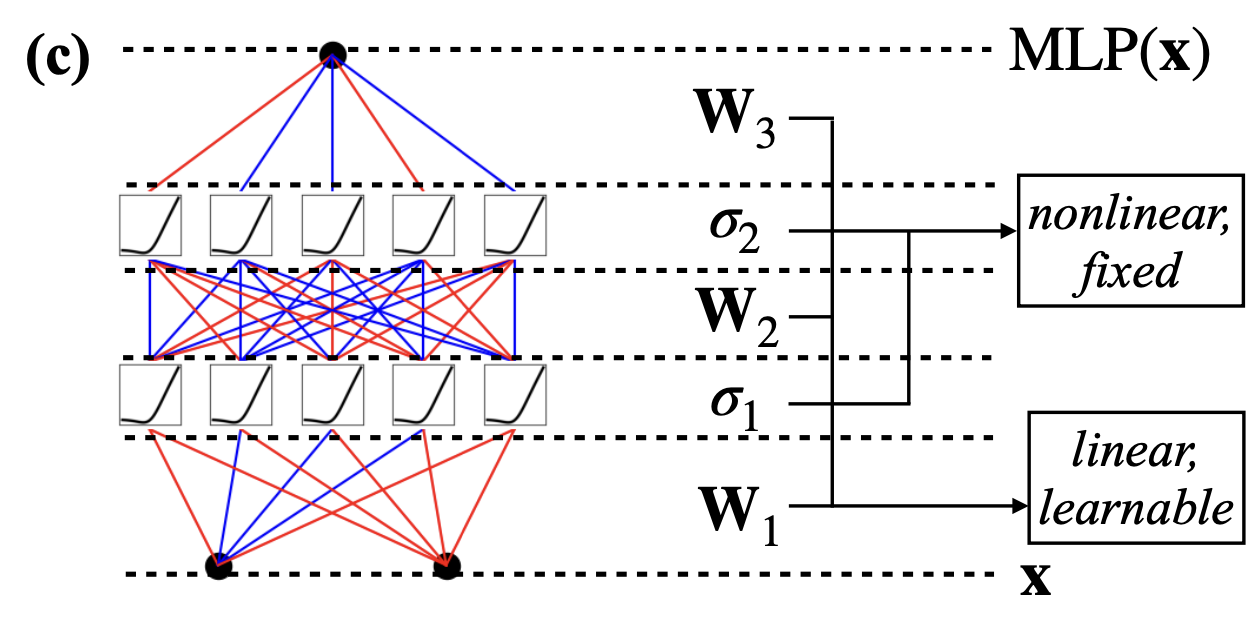
\includegraphics[width=6cm]{deepmlp}}{\textit{A deep multi-layer perceptron.}}
\end{frame}
\begin{frame}
    \[
        \hat{f}(x) =  \sum_i^{N(\varepsilon)} a_i \sigma \left[\mathbf{W}_i \mathbf{x} + b_i \right]
    \]
    \textbf{\textit{Question:}} What can a multi-layer perceptron represent? \\
    \textbf{\textit{Answer}} Anything!$^*$ \\
\end{frame}
\begin{frame}
    \textbf{\textit{Question:}} What can a multi-layer perceptron represent? \\
    \textbf{\textit{Answer}} Anything!$^*$ \\
    \vspace{1cm}
    Let $D \subset \R^n$ be compact\footnote{\tiny
        Compact denotes some notion of ``closed and bounded'' -- the $n$-dimensional
        equivalent of a closed interval $[a, b] \subset \R$.
    }.
    $f: D \longrightarrow \R$ be an \textit{arbitrary nonlinear function}, and let $\hat{f}: D \longrightarrow
    \R$ denote a shallow (\textit{n.b.} 2-layer) multi-layer perceptron, denoted by
    \[
        \hat{f}(x) =  \sum_i^{N(\varepsilon)} a_i \sigma \left[\mathbf{W}_i \mathbf{x} + b_i \right]
    \]
    where $N(\varepsilon)$ is the \textit{number of neurons}. In the shallow case this is $=$ 
    the width.
\end{frame}
\begin{frame}
    Let $D \subset \R^n$ be compact.
    $f: D \longrightarrow \R$ be an \textit{arbitrary nonlinear function}, and let $\hat{f}: D \longrightarrow
    \R$ denote a shallow (\textit{n.b.} 2-layer) multi-layer perceptron, denoted by
    \[
        \hat{f}(x) =  \sum_i^{N(\varepsilon)} a_i \sigma \left[\mathbf{W}_i \mathbf{x} + b_i \right]
    \]
    \begin{theorem}
        \textbf{Universal approximation (2-layer network).} For arbitrary $\varepsilon \in \R > 0$, there
        exists $N(\varepsilon)$ such that 
        \[
        |f(x) - \hat{f(x)}| \leq \varepsilon
        \]
    \end{theorem}
\end{frame}

\begin{frame}
    \[
        \hat{f}(x) =  \sum_i^{N(\varepsilon)} a_i \sigma \left[\mathbf{W}_i \mathbf{x} + b_i \right]
    \]
    \begin{theorem}
        \textbf{Universal approximation (2-layer network).} For arbitrary $\varepsilon \in \R > 0$, there
        exists $N(\varepsilon)$ such that 
        \[
        |f(x) - \hat{f(x)}| \leq \varepsilon
        \]
    \end{theorem}
    So we can model basically anything! But...
\end{frame}

\begin{frame}
    \begin{theorem}
        \textbf{Universal approximation (2-layer network).} For arbitrary $\varepsilon \in \R > 0$, there
        exists $N(\varepsilon)$ such that 
        \[
        |f(x) - \hat{f(x)}| \leq \varepsilon
        \]
    \end{theorem}
    The million-dollar question:
    \begin{center}
        \textbf{What is $N(\varepsilon)$?}
    \end{center}
\end{frame}
\begin{frame}
    \center{ \textbf{What is $N(\varepsilon)$?} }
    \\
    \textbf{We don't know, in general!} The universal approximation theorem guarantees no bounds on $N$. 
    For deep networks,
    we do know that it's possibly poorly behaved ($N \propto \exp(d)$, the layer depth of the network).
\end{frame}

\begin{frame}
    \textbf{Why does this make sense?} Because we are fitting a ``mostly linear'' model to an ``arbitrary
    non-linear'' function. We need ``a lot of linear pieces'' to get good at modeling funky nonlinear functions.

    \ffig{
        \begin{tikzpicture}[yscale=0.3]
            \begin{scope}
                \draw[red,thick,->] plot [domain=-3.3:3.3] ({\x}, {\x * \x});
                % \draw (3, 9) node [above right] (quad) {x^2};
            \end{scope}
            \draw[blue, <-] (3, 9) -- (2, 4) -- (1, 1) -- (0, 0) -- (-1, 1) -- (-2, 4) -- (-3, 9);
            \draw[->] (-4.8, 0) -- (4.8, 0);
            \draw[->] (0, -1.8) -- (0, 10.8);
            \draw[step=2cm,very thin,color=gray] (-4.1, -1.1) grid (4.1, 10.1);
            \draw[--] (-3, 0.3) -- (-3, -0.3) node [below=1mm] {-3};
            \draw[--] (3, 0.3) -- (3, -0.3) node [below=1mm] {3};
            \draw (3, 9) node [above,right=2mm,fill=white] (quad) {$f = x^2$};
        \end{tikzpicture}
    }{\textit{It takes a lot of line segments to approximate this quadratic, and as soon as we leave $[-3, 3]$,
    the error in our approximation blows up!}}

    Enter the notion of \textit{neural scaling laws}.
\end{frame}

\begin{frame}
    Neural scaling laws formalize the notion of ``mostly linear things approximate nonlinearities inefficiently'' --
    we can generally say that the \textit{training}\footnote{
        i.e. overfits
    } loss $\ell$ decreases according to 
    \[
        \ell \propto N^{-\alpha}
    \]
    where $\alpha$ is the \textit{scaling exponent}. 
\end{frame}

\end{document}
